\documentclass[9pt]{beamer}
\usepackage[utf8]{inputenc}
\usepackage{tikz, pgfplots}
\pgfplotsset{compat=1.18}
\usetikzlibrary{positioning}
\usetikzlibrary{trees}
\usetikzlibrary{shapes.geometric, arrows.meta, positioning}
\usepackage{xcolor}
\usepackage{graphicx}
\usepackage{subcaption}
\usepackage{hyperref} 
\usepackage{colortbl} % Required for \rowcolor
\usepackage{animate}
\usepackage{asymptote}
\usepackage[T1]{fontenc}
\usepackage{amsmath, amsfonts, amssymb}
\usepackage{cancel}
\usepackage[french]{babel}
\usepackage[normalem]{ulem}

% Reduce only the slide body text size (leave titles at theme defaults)
\setbeamerfont{normal text}{size=\small}

% Theme và màu sắc cho beamer
\usetheme{AnnArbor}
\usecolortheme{seahorse}

% Định nghĩa và thiết lập màu sắc chung
\definecolor{mydarkblue}{RGB}{0,51,102}
\setbeamercolor{structure}{fg=mydarkblue}
\setbeamercolor{frametitle}{bg=mydarkblue, fg=white}
\setbeamercolor{title}{fg=mydarkblue}
\setbeamercolor{item}{fg=mydarkblue}
\setbeamercolor{block title}{bg=mydarkblue, fg=white}
\setbeamercolor{block body}{bg=white, fg=black}
\setbeamercolor{section in toc}{fg=mydarkblue}
\setbeamercolor{subsection in toc}{fg=mydarkblue}
\setbeamercolor{caption name}{fg=mydarkblue}
\setbeamercolor{author}{fg=mydarkblue}
\setbeamercolor{date}{fg=mydarkblue}
\setbeamercolor{institute}{fg=mydarkblue}
\setbeamertemplate{caption}[numbered]
\usepackage{multirow}
\title{PIC anormale}
\author{Viet Anh Quach}
\institute{3SR}
\date{\today}

\begin{document}


\section{DEM}
% \begin{frame}{Modèle: Triaxiale selon l'axe y}
%         \centering
%     \begin{figure}
%     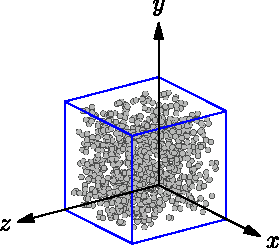
\includegraphics[width=0.5\textwidth]{modele.pdf}
%     \end{figure}
%     % Générer picAbnormale-1.pdf avec Asymptote séparément, puis compiler ce fichier
%     Condition de limite: Périodique
% \end{frame}

% \begin{frame}{Paramètres d'échantillon}
%     \begin{table}
%         \centering
%         \begin{tabular}{|c|c|c|c|}
%             \hline
%             \textbf{Symboles}               & \textbf{Paramètres}         & \textbf{Valeurs}                          & \textbf{Unité}  \\
%             \hline
%             Nombre de particules            & N                           & $1000$                                    & -               \\
%             \hline
%             Le rayon des particules         & R                           & 0.003 $\div$ 0.005                        & m               \\
%             \hline
%             Masse volumique                 & $\rho$                      & 2500                                      & $\text{kg/m}^3$ \\
%             \hline
%             Contrainte isotrope             & $\sigma_{xx} = \sigma_{zz}$ & 30                             & kPa             \\
%             \hline
%             Raideur normale et tangentielle & $k_n$ \& $k_t$              & \textcolor{black}{$3 \times 10^6$}        & $\text{N/m}$    \\
%             \hline
%             Niveau de raideur               & $\kappa$                    & 6250                                      & -               \\
%             \hline
%             Coefficient de frottement       & $\mu_{isotrope} = \mu_{triaxiale}$                       & 0.5                                       & -               \\
%             \hline
%             Masse de la cellule périodique  & $h_{mass}$                  & \textcolor{black}{$7.13 \times 10^{-4}$}  & $\text{kg}$     \\
%             \hline
%             Nombre d’inertie                & I                           & \textcolor{red}{$10^{-4}\  \div \ 10^{-2}$} & -               \\
%             \hline
%             Pas de temps                    & $d_t$                       & $10^{-6}\  \div \ 10^{-9}$                 & $\text{s}$      \\
%             \hline
%             Coefficient d'amortissement     & $\alpha$                    & \textcolor{black}{0}       & -               \\
%             \hline
%         \end{tabular}
%         \caption{Valeurs des paramètres utilisés dans la compression triaxiale}
%     \end{table}
% \end{frame}

% \begin{frame}{PIC anormale}
%     \begin{columns}
%         \begin{column}{0.5\textwidth}
%             \begin{figure}
%                 \centering
%                 \scalebox{0.5}{% GNUPLOT: LaTeX picture with Postscript
\begingroup
  \makeatletter
  \providecommand\color[2][]{%
    \GenericError{(gnuplot) \space\space\space\@spaces}{%
      Package color not loaded in conjunction with
      terminal option `colourtext'%
    }{See the gnuplot documentation for explanation.%
    }{Either use 'blacktext' in gnuplot or load the package
      color.sty in LaTeX.}%
    \renewcommand\color[2][]{}%
  }%
  \providecommand\includegraphics[2][]{%
    \GenericError{(gnuplot) \space\space\space\@spaces}{%
      Package graphicx or graphics not loaded%
    }{See the gnuplot documentation for explanation.%
    }{The gnuplot epslatex terminal needs graphicx.sty or graphics.sty.}%
    \renewcommand\includegraphics[2][]{}%
  }%
  \providecommand\rotatebox[2]{#2}%
  \@ifundefined{ifGPcolor}{%
    \newif\ifGPcolor
    \GPcolortrue
  }{}%
  \@ifundefined{ifGPblacktext}{%
    \newif\ifGPblacktext
    \GPblacktextfalse
  }{}%
  % define a \g@addto@macro without @ in the name:
  \let\gplgaddtomacro\g@addto@macro
  % define empty templates for all commands taking text:
  \gdef\gplbacktext{}%
  \gdef\gplfronttext{}%
  \makeatother
  \ifGPblacktext
    % no textcolor at all
    \def\colorrgb#1{}%
    \def\colorgray#1{}%
  \else
    % gray or color?
    \ifGPcolor
      \def\colorrgb#1{\color[rgb]{#1}}%
      \def\colorgray#1{\color[gray]{#1}}%
      \expandafter\def\csname LTw\endcsname{\color{white}}%
      \expandafter\def\csname LTb\endcsname{\color{black}}%
      \expandafter\def\csname LTa\endcsname{\color{black}}%
      \expandafter\def\csname LT0\endcsname{\color[rgb]{1,0,0}}%
      \expandafter\def\csname LT1\endcsname{\color[rgb]{0,1,0}}%
      \expandafter\def\csname LT2\endcsname{\color[rgb]{0,0,1}}%
      \expandafter\def\csname LT3\endcsname{\color[rgb]{1,0,1}}%
      \expandafter\def\csname LT4\endcsname{\color[rgb]{0,1,1}}%
      \expandafter\def\csname LT5\endcsname{\color[rgb]{1,1,0}}%
      \expandafter\def\csname LT6\endcsname{\color[rgb]{0,0,0}}%
      \expandafter\def\csname LT7\endcsname{\color[rgb]{1,0.3,0}}%
      \expandafter\def\csname LT8\endcsname{\color[rgb]{0.5,0.5,0.5}}%
    \else
      % gray
      \def\colorrgb#1{\color{black}}%
      \def\colorgray#1{\color[gray]{#1}}%
      \expandafter\def\csname LTw\endcsname{\color{white}}%
      \expandafter\def\csname LTb\endcsname{\color{black}}%
      \expandafter\def\csname LTa\endcsname{\color{black}}%
      \expandafter\def\csname LT0\endcsname{\color{black}}%
      \expandafter\def\csname LT1\endcsname{\color{black}}%
      \expandafter\def\csname LT2\endcsname{\color{black}}%
      \expandafter\def\csname LT3\endcsname{\color{black}}%
      \expandafter\def\csname LT4\endcsname{\color{black}}%
      \expandafter\def\csname LT5\endcsname{\color{black}}%
      \expandafter\def\csname LT6\endcsname{\color{black}}%
      \expandafter\def\csname LT7\endcsname{\color{black}}%
      \expandafter\def\csname LT8\endcsname{\color{black}}%
    \fi
  \fi
    \setlength{\unitlength}{0.0500bp}%
    \ifx\gptboxheight\undefined%
      \newlength{\gptboxheight}%
      \newlength{\gptboxwidth}%
      \newsavebox{\gptboxtext}%
    \fi%
    \setlength{\fboxrule}{0.5pt}%
    \setlength{\fboxsep}{1pt}%
    \definecolor{tbcol}{rgb}{1,1,1}%
\begin{picture}(7200.00,5040.00)%
    \gplgaddtomacro\gplbacktext{%
      \csname LTb\endcsname%%
      \put(814,1144){\makebox(0,0)[r]{\strut{}$0$}}%
      \csname LTb\endcsname%%
      \put(814,1512){\makebox(0,0)[r]{\strut{}$20$}}%
      \csname LTb\endcsname%%
      \put(814,1879){\makebox(0,0)[r]{\strut{}$40$}}%
      \csname LTb\endcsname%%
      \put(814,2247){\makebox(0,0)[r]{\strut{}$60$}}%
      \csname LTb\endcsname%%
      \put(814,2614){\makebox(0,0)[r]{\strut{}$80$}}%
      \csname LTb\endcsname%%
      \put(814,2982){\makebox(0,0)[r]{\strut{}$100$}}%
      \csname LTb\endcsname%%
      \put(814,3349){\makebox(0,0)[r]{\strut{}$120$}}%
      \csname LTb\endcsname%%
      \put(814,3717){\makebox(0,0)[r]{\strut{}$140$}}%
      \csname LTb\endcsname%%
      \put(814,4084){\makebox(0,0)[r]{\strut{}$160$}}%
      \csname LTb\endcsname%%
      \put(814,4452){\makebox(0,0)[r]{\strut{}$180$}}%
      \csname LTb\endcsname%%
      \put(814,4819){\makebox(0,0)[r]{\strut{}$200$}}%
      \csname LTb\endcsname%%
      \put(946,924){\makebox(0,0){\strut{}$0$}}%
      \csname LTb\endcsname%%
      \put(1968,924){\makebox(0,0){\strut{}$10$}}%
      \csname LTb\endcsname%%
      \put(2990,924){\makebox(0,0){\strut{}$20$}}%
      \csname LTb\endcsname%%
      \put(4011,924){\makebox(0,0){\strut{}$30$}}%
      \csname LTb\endcsname%%
      \put(5033,924){\makebox(0,0){\strut{}$40$}}%
      \csname LTb\endcsname%%
      \put(6055,924){\makebox(0,0){\strut{}$50$}}%
      \put(6187,1144){\makebox(0,0)[l]{\strut{}$-2$}}%
      \put(6187,1512){\makebox(0,0)[l]{\strut{}$-1$}}%
      \put(6187,1879){\makebox(0,0)[l]{\strut{}$0$}}%
      \put(6187,2247){\makebox(0,0)[l]{\strut{}$1$}}%
      \put(6187,2614){\makebox(0,0)[l]{\strut{}$2$}}%
      \put(6187,2982){\makebox(0,0)[l]{\strut{}$3$}}%
      \put(6187,3349){\makebox(0,0)[l]{\strut{}$4$}}%
      \put(6187,3717){\makebox(0,0)[l]{\strut{}$5$}}%
      \put(6187,4084){\makebox(0,0)[l]{\strut{}$6$}}%
      \put(6187,4452){\makebox(0,0)[l]{\strut{}$7$}}%
      \put(6187,4819){\makebox(0,0)[l]{\strut{}$8$}}%
    }%
    \gplgaddtomacro\gplfronttext{%
      \csname LTb\endcsname%%
      \put(341,2981){\rotatebox{-270}{\makebox(0,0){\strut{}q (kPa)}}}%
      \put(6693,2981){\rotatebox{-270}{\makebox(0,0){\strut{}$\varepsilon_v$ (\%)}}}%
      \put(3500,594){\makebox(0,0){\strut{}$\varepsilon_{yy}$ (\%)}}%
      \csname LTb\endcsname%%
      \put(2645,393){\makebox(0,0)[r]{\strut{}$I = 10^{-4}$}}%
      \csname LTb\endcsname%%
      \put(2645,173){\makebox(0,0)[r]{\strut{}$I = 10^{-3}$}}%
      \csname LTb\endcsname%%
      \put(4556,393){\makebox(0,0)[r]{\strut{}$I = 10^{-2}$}}%
      \csname LTb\endcsname%%
      \put(4556,173){\makebox(0,0)[r]{\strut{}$I = 10^{-1}$}}%
    }%
    \gplbacktext
    \put(0,0){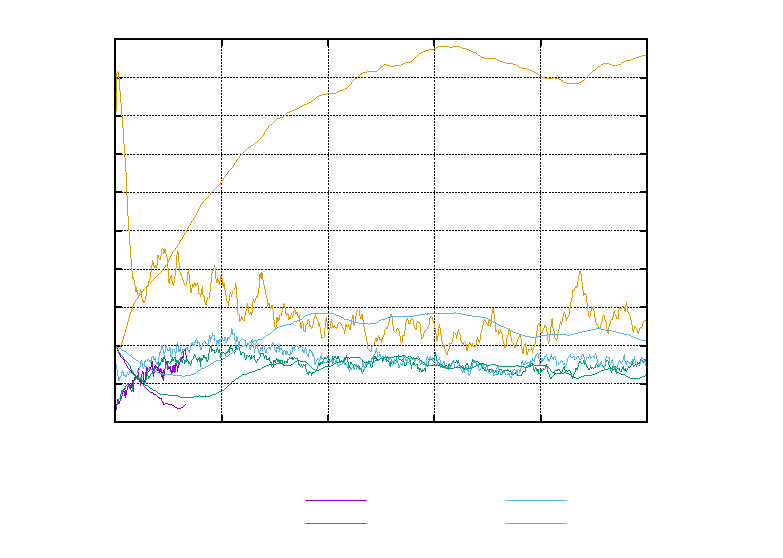
\includegraphics[width={360.00bp},height={252.00bp}]{./1000KineticComp}}%
    \gplfronttext
  \end{picture}%
\endgroup
}
%                 \caption{Contrainte déviatorique}
%             \end{figure}
%         \end{column}
%         \begin{column}{0.5\textwidth}
%             \begin{figure}
%                 \centering
%                 \scalebox{0.5}{% GNUPLOT: LaTeX picture with Postscript
\begingroup
  \makeatletter
  \providecommand\color[2][]{%
    \GenericError{(gnuplot) \space\space\space\@spaces}{%
      Package color not loaded in conjunction with
      terminal option `colourtext'%
    }{See the gnuplot documentation for explanation.%
    }{Either use 'blacktext' in gnuplot or load the package
      color.sty in LaTeX.}%
    \renewcommand\color[2][]{}%
  }%
  \providecommand\includegraphics[2][]{%
    \GenericError{(gnuplot) \space\space\space\@spaces}{%
      Package graphicx or graphics not loaded%
    }{See the gnuplot documentation for explanation.%
    }{The gnuplot epslatex terminal needs graphicx.sty or graphics.sty.}%
    \renewcommand\includegraphics[2][]{}%
  }%
  \providecommand\rotatebox[2]{#2}%
  \@ifundefined{ifGPcolor}{%
    \newif\ifGPcolor
    \GPcolortrue
  }{}%
  \@ifundefined{ifGPblacktext}{%
    \newif\ifGPblacktext
    \GPblacktextfalse
  }{}%
  % define a \g@addto@macro without @ in the name:
  \let\gplgaddtomacro\g@addto@macro
  % define empty templates for all commands taking text:
  \gdef\gplbacktext{}%
  \gdef\gplfronttext{}%
  \makeatother
  \ifGPblacktext
    % no textcolor at all
    \def\colorrgb#1{}%
    \def\colorgray#1{}%
  \else
    % gray or color?
    \ifGPcolor
      \def\colorrgb#1{\color[rgb]{#1}}%
      \def\colorgray#1{\color[gray]{#1}}%
      \expandafter\def\csname LTw\endcsname{\color{white}}%
      \expandafter\def\csname LTb\endcsname{\color{black}}%
      \expandafter\def\csname LTa\endcsname{\color{black}}%
      \expandafter\def\csname LT0\endcsname{\color[rgb]{1,0,0}}%
      \expandafter\def\csname LT1\endcsname{\color[rgb]{0,1,0}}%
      \expandafter\def\csname LT2\endcsname{\color[rgb]{0,0,1}}%
      \expandafter\def\csname LT3\endcsname{\color[rgb]{1,0,1}}%
      \expandafter\def\csname LT4\endcsname{\color[rgb]{0,1,1}}%
      \expandafter\def\csname LT5\endcsname{\color[rgb]{1,1,0}}%
      \expandafter\def\csname LT6\endcsname{\color[rgb]{0,0,0}}%
      \expandafter\def\csname LT7\endcsname{\color[rgb]{1,0.3,0}}%
      \expandafter\def\csname LT8\endcsname{\color[rgb]{0.5,0.5,0.5}}%
    \else
      % gray
      \def\colorrgb#1{\color{black}}%
      \def\colorgray#1{\color[gray]{#1}}%
      \expandafter\def\csname LTw\endcsname{\color{white}}%
      \expandafter\def\csname LTb\endcsname{\color{black}}%
      \expandafter\def\csname LTa\endcsname{\color{black}}%
      \expandafter\def\csname LT0\endcsname{\color{black}}%
      \expandafter\def\csname LT1\endcsname{\color{black}}%
      \expandafter\def\csname LT2\endcsname{\color{black}}%
      \expandafter\def\csname LT3\endcsname{\color{black}}%
      \expandafter\def\csname LT4\endcsname{\color{black}}%
      \expandafter\def\csname LT5\endcsname{\color{black}}%
      \expandafter\def\csname LT6\endcsname{\color{black}}%
      \expandafter\def\csname LT7\endcsname{\color{black}}%
      \expandafter\def\csname LT8\endcsname{\color{black}}%
    \fi
  \fi
    \setlength{\unitlength}{0.0500bp}%
    \ifx\gptboxheight\undefined%
      \newlength{\gptboxheight}%
      \newlength{\gptboxwidth}%
      \newsavebox{\gptboxtext}%
    \fi%
    \setlength{\fboxrule}{0.5pt}%
    \setlength{\fboxsep}{1pt}%
    \definecolor{tbcol}{rgb}{1,1,1}%
\begin{picture}(7200.00,5040.00)%
    \gplgaddtomacro\gplbacktext{%
      \csname LTb\endcsname%%
      \put(682,1584){\makebox(0,0)[r]{\strut{}$-2$}}%
      \csname LTb\endcsname%%
      \put(682,1908){\makebox(0,0)[r]{\strut{}$-1$}}%
      \csname LTb\endcsname%%
      \put(682,2231){\makebox(0,0)[r]{\strut{}$0$}}%
      \csname LTb\endcsname%%
      \put(682,2555){\makebox(0,0)[r]{\strut{}$1$}}%
      \csname LTb\endcsname%%
      \put(682,2878){\makebox(0,0)[r]{\strut{}$2$}}%
      \csname LTb\endcsname%%
      \put(682,3202){\makebox(0,0)[r]{\strut{}$3$}}%
      \csname LTb\endcsname%%
      \put(682,3525){\makebox(0,0)[r]{\strut{}$4$}}%
      \csname LTb\endcsname%%
      \put(682,3849){\makebox(0,0)[r]{\strut{}$5$}}%
      \csname LTb\endcsname%%
      \put(682,4172){\makebox(0,0)[r]{\strut{}$6$}}%
      \csname LTb\endcsname%%
      \put(682,4496){\makebox(0,0)[r]{\strut{}$7$}}%
      \csname LTb\endcsname%%
      \put(682,4819){\makebox(0,0)[r]{\strut{}$8$}}%
      \csname LTb\endcsname%%
      \put(814,1364){\makebox(0,0){\strut{}$0$}}%
      \csname LTb\endcsname%%
      \put(2012,1364){\makebox(0,0){\strut{}$10$}}%
      \csname LTb\endcsname%%
      \put(3210,1364){\makebox(0,0){\strut{}$20$}}%
      \csname LTb\endcsname%%
      \put(4407,1364){\makebox(0,0){\strut{}$30$}}%
      \csname LTb\endcsname%%
      \put(5605,1364){\makebox(0,0){\strut{}$40$}}%
      \csname LTb\endcsname%%
      \put(6803,1364){\makebox(0,0){\strut{}$50$}}%
    }%
    \gplgaddtomacro\gplfronttext{%
      \csname LTb\endcsname%%
      \put(209,3201){\rotatebox{-270}{\makebox(0,0){\strut{}$\varepsilon_v$ (\%)}}}%
      \put(3808,1034){\makebox(0,0){\strut{}$\varepsilon_{yy}$ (\%)}}%
      \csname LTb\endcsname%%
      \put(2953,833){\makebox(0,0)[r]{\strut{}$I = 10^{-4}$}}%
      \csname LTb\endcsname%%
      \put(2953,613){\makebox(0,0)[r]{\strut{}$I = 10^{-3}$}}%
      \csname LTb\endcsname%%
      \put(2953,393){\makebox(0,0)[r]{\strut{}$I = 10^{-2}$}}%
      \csname LTb\endcsname%%
      \put(2953,173){\makebox(0,0)[r]{\strut{}$I = 2 \times 10^{-2}$}}%
      \csname LTb\endcsname%%
      \put(5392,833){\makebox(0,0)[r]{\strut{}$I = 4 \times 10^{-2}$}}%
      \csname LTb\endcsname%%
      \put(5392,613){\makebox(0,0)[r]{\strut{}$I = 6 \times 10^{-2}$}}%
      \csname LTb\endcsname%%
      \put(5392,393){\makebox(0,0)[r]{\strut{}$I = 8 \times 10^{-2}$}}%
      \csname LTb\endcsname%%
      \put(5392,173){\makebox(0,0)[r]{\strut{}$I = 10^{-1}$}}%
    }%
    \gplbacktext
    \put(0,0){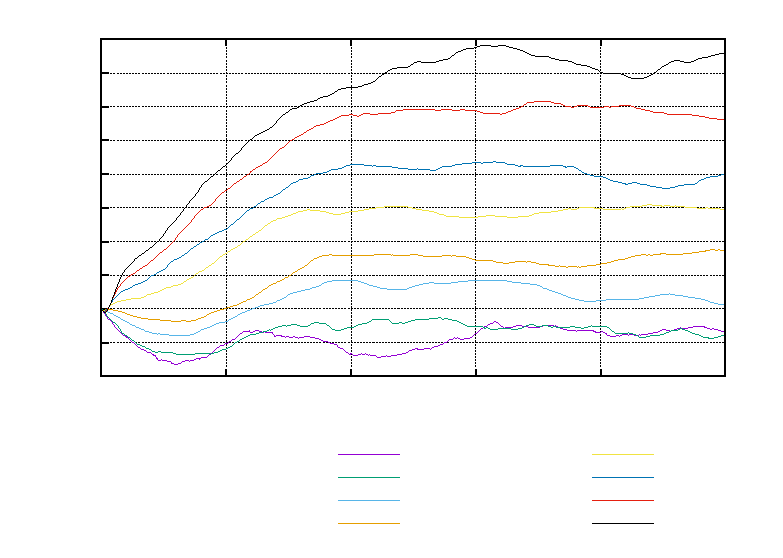
\includegraphics[width={360.00bp},height={252.00bp}]{./1000Deformation}}%
    \gplfronttext
  \end{picture}%
\endgroup
}
%                 \caption{Déformation Volumique}
%             \end{figure}
%         \end{column}
%     \end{columns}
% \end{frame}

\begin{frame}{Nombre d'Inertie}
    Le nombre d'inerties "I" est défini à partir du ``temps d'inertie'' et du ``temps de cisaillement''.
    Le temps d'inertie caractérise le temps de déplacement d'une particule moyenne de masse $m$ et de diamètre $d$, sous la pression $P$, dans $D$ dimensions\footnote{Lecture \textit{Discrete Element Modeling} – Gaël COMBE}. Leurs expressions sont :
    \begin{align}
        	\tau_c &= \dfrac{1}{\dot{\epsilon}} = \dfrac{v}{H_0}, \\
        	\tau_i &= \sqrt{\dfrac{m}{P d^{D-2}}} .
    \end{align}

    Dans notre cas (compression triaxiale en 3D, $D=3$) on obtient :
    \begin{align}
        I &= \dfrac{\tau_i}{\tau_c}
        = \dfrac{v}{H_0}\,\sqrt{\dfrac{\tfrac{4}{3}\pi R^3 \rho}{\sigma_{0}\times 2R}} \,.
    \end{align}

    Où :
    \begin{itemize}
        \item $v$ : vitesse de compression,
        \item $H_0$ : hauteur initiale de l'échantillon,
        \item $R$ : rayon moyen des particules et $\rho$ : leaur masse volumique 
        \item $\sigma_{0}$ : contrainte de confinement
    \end{itemize}
\end{frame}



\end{document}
